\chapter{Grundlagen}

Das nachfolgende Kapitel beschreibt die Grundlagen, welche in dieser Arbeit benötigt werden. Es besteht aus drei Abschnitten. Im ersten Abschnitt wird auf die Darstellung von kontinuierlich-sinusförmige Signale und deren Einheiten sowie die Schreibweise von Gleichungen eingegangen. Der zweite Abschnitt stellt die Kommunikationsprotokolle und deren Schichtenmodelle dar. Die BSD-Sockets werden im letzten Abschnitt erläutert. Außerdem umfasst der letzte Teil auch die Herstellung der Kommunikation mittels BSD-Sockets.

\section{Elektrotechnische Grundlagen}
In der Elektrotechnik wird die elektrische Energie entweder als Gleichstrom oder als Wechselstrom übertragen. Beim Gleichstrom ändern sich weder die Stärke noch die Richtung, aber beim Wechselstrom sind die Stärke und die Richtung im zeitlichen Verlauf veränderlich. Die einfache Erzeugung der Wechselspannung ist mit den elektromagnetischen Motoren möglich, welche rotierende Maschinen sind. Die Richtung der magnetischen Feldlinien ändert sich in einer Spule, dann wird eine Wechselspannung in diese sich drehenden Maschine induziert. \smallskip \smallskip

\begin{figure}[htbp]
	\centering
	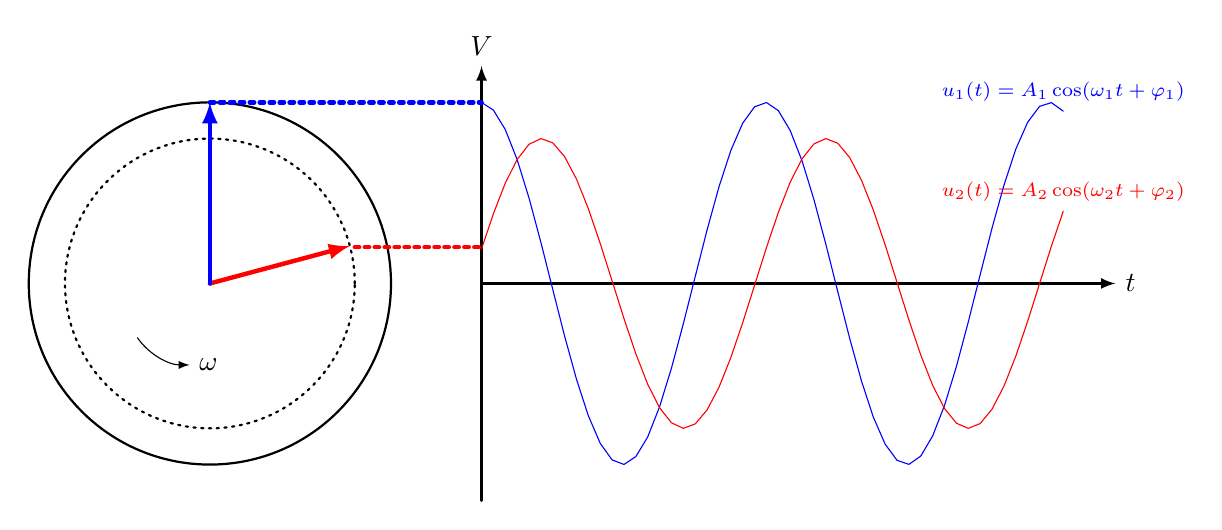
\begin{tikzpicture}[scale=2.3,cap=round,>=latex]
	
	        % draw the coordinates
%		\draw[->] (-1.2cm,0cm) -- (1.2cm,0cm) node[right,fill=white] {$\Re e$};
%     		\draw[->] (0cm,-1.2cm) -- (0cm,1.2cm) node[above,fill=white] {$\Im m$};

		% draw the unit circle
		\draw[thick] (0cm,0cm) circle(1cm);
		\draw[thick] [dotted] (0cm,0cm) circle(0.8 cm);
		
                	% lines from center to point
		\draw[red] [ultra thick] [->] (0cm,0cm) -- (15:0.8cm);
		\draw[blue] [ultra thick] [->] (0cm,0cm) -- (90:1cm);

		%Raster zeichnen
%		\draw [color=gray!50]  [step=5mm] (0,-2) grid (10,2);
		% Achsen zeichnen
		\draw[->,thick] (1.5,0) -- (5,0) node[right] {$t$};
		\draw[->,thick] (1.5,-1.2) -- (1.5,1.2) node[above] {$V$};
		
		% Pfeile 
		\draw[red] [dotted, ultra thick] (0.8,0.2) -- (1.5,0.2);
		\draw[blue] [dotted, ultra thick] (0,1) -- (1.5,1);

		% cos
		%\draw [red,domain=1.5:pi] plot (\x, {0.8*cos(4 * \x r + 0.4*pi)});
		\draw [blue,domain=1.5:1.5*pi,samples=50] plot (\x, {cos(((4*\x)+pi/10) r)})node[above]{\scriptsize $u_1(t) = A_1 \cos (\omega_1 t + \varphi_1)$};
		\draw [red,domain=1.5:1.5*pi,samples=50] plot (\x, {-0.8*cos(4*(\x+pi/6) r)})node[above]{\scriptsize $u_2(t) = A_2 \cos (\omega_2 t + \varphi_2)$};
		
		% w
		\draw [->] (-0.4,-0.3) arc (215:270:10pt)node[right]{$\omega$};

	\end{tikzpicture}
	\caption{Kontinuierlich-sinusförmige Signale} \label{fig:signal}
\end{figure}

Wie in der \autoref{fig:signal} zu sehen ist, kann eine Wechselspannung bzw. ein Wechselstrom mit dem winkelförmigen Zeiger erzeugt werden, wobei so ein Signal auch als ein kontinuierlich-sinusförmiges Signal bezeichnet werden. Als allgemeine Form wird eine Wechselspannung bzw. ein kontinuierlich-sinusförmiges Signal mathematisch

\begin{align}
	u(t) = A \cos (\omega t + \varphi)
	\label{signal:math}
\end{align}

mit den folgenden Parametern beschrieben: 

\begin{itemize}
	\item $A$: Amplitude der Wechselgröße ($Volt$)
	\item $\omega$: Kreisfrequenz mit $\omega = 2 \pi f$ ($Radius/sek.$)
	\item $f$: Frequenz ($T^{-1}$ Hz)
	\item $T$: Period ($1/f$ sek.)
	\item $\varphi$: Phase ($Radius$)
\end{itemize}

In der Signalverarbeitung können die Signale mit verschiedenen Operationen verarbeitet werden. Zum Beispiel können zwei oder mehrere Signale addiert bzw. multipliziert werden. Außerdem können auch die Parameter dieser Signale geändert werden. \smallskip \smallskip

Es sind zwei verschiedene Lösungswege möglich. Entweder kann die Lösung mittels geometrischer oder mittels algebraischer Methode gefunden werden, wobei die geometrische Methode der schwierigere Ansatz ist. Der algebraische Ansatz wird mit Hilfe der eulerschen Formel\footnote{besagt, dass eine trigonometrische Funktion als Exponentialfunktion auch gebildet werden kann: \\ $A e^{j(\omega t + \varphi)} = A \cos(\omega t + \varphi) + j A \sin(\omega t + \varphi)$} analysiert. \smallskip \smallskip

%Gegeben seien beispielsweise folgende drei Signale, die mit den verschiedenen Parametern zu addieren sind:

%\begin{itemize}
%	\item $u_1(t) = 10 \cos (2 \pi t)$
%	\item $u_2(t) =  \frac{1}{2} u_1(t - \frac{\pi}{4}) = 5 \cos(2 \pi t - \frac{\pi}{2})$
%	\item $u_3(t) =  -\frac{1}{2} u_1(-t + \frac{\pi}{4}) = -5 \cos(-2 \pi t + \frac{\pi}{2})$
%\end{itemize}

Die trigonometrische Funktionen werden als imaginäre Exponentionalfunktionen dargestellt, wie im Folgenden beschrieben wird:

\begin{align}
	\cos (\omega t + \varphi) = \frac{e^{j(\omega t + \varphi)} + e^{-j(\omega t + \varphi)}}{2}\label{euler:cos}
\end{align}

\begin{align}
	\sin (\omega t + \varphi) = \frac{e^{j(\omega t + \varphi)} - e^{-j(\omega t + \varphi)}}{2j}\label{euler:sin}
\end{align}
\smallskip \smallskip

%Gemäß der \autoref{euler:cos} sind die Signale $u_1$, $u_2$ und $u_3$ in die eulerschen Form umgeformt, wie folgt dargestellt:

%\begin{itemize}
%	\item $u_1 = 10  \frac{e^{j 2 \pi t} + e^{-j 2 \pi t}}{2} $
%	\item $u_2 = 5 \frac{e^{j (2 \pi t - \frac{\pi}{2})} + e^{-j (2 \pi t - \frac{\pi}{2})}}{2}$
%	\item $u_3 = -5 \frac{e^{j (-2 \pi t + \frac{\pi}{2})} + e^{-j (-2 \pi t + \frac{\pi}{2})}}{2}$
%\end{itemize}

%Anschließend ergibt sich die Summe dieser drei Signale wie folgt: \\

%$u_1(t) + u_2(t) + u_3(t) = 10  \frac{e^{j 2 \pi t} + e^{-j 2 \pi t}}{2} + 5 \frac{e^{j (2 \pi t - \frac{\pi}{2})} + e^{-j (2 \pi t - \frac{\pi}{2})}}{2} -5 \frac{e^{j (-2 \pi t + \frac{\pi}{2})} + e^{-j (-2 \pi t + \frac{\pi}{2})}}{2} $ \\

%$=  \frac{10 e^{j 2 \pi t} + 10 e^{-j 2 \pi t} + 5 e^{j (2 \pi t - \frac{\pi}{2})} + 5 e^{-j (2 \pi t - \frac{\pi}{2})} - 5 e^{j (-2 \pi t + \frac{\pi}{2})} - 5 e^{-j (-2 \pi t + \frac{\pi}{2})}}{2}$ \\

%$=	\frac{10 e^{j 2 \pi t} + 10 e^{-j 2 \pi t} 
%	+ \overbrace{ 5 e^{j (2 \pi t - \frac{\pi}{2})}}^{Term A} 
%	+  \overbrace{ 5 e^{j (-2 \pi t + \frac{\pi}{2})}}^{Term B} 
%	-  \overbrace{ 5 e^{j (-2 \pi t + \frac{\pi}{2})}}^{Term B}
%	- \overbrace{ 5 e^{j (2 \pi t - \frac{\pi}{2})}}^{Term A}
%	}{2}
%$ \\

%Wie in der letzten Zeile zu sehen ist, werden die \textbf{Terme A} und \textbf{B} in der Berechnung entfernt. Danach ist das Ergebnis wie folgt: \\

%$
%= \frac{10 e^{j 2 \pi t} + 10 e^{-j 2 \pi t}}{2} = 10 \cos(2 \pi t)
%$ \\

In dieser Arbeit wird ein kontinuierlich-sinusförmiges Eingangssignal mit Hilfe eines Optokopplers als kontinuierlich-rechteckförmiges Ausgangssignal repräsentiert bzw. umgeformt, weil die fallenden und/oder steigenden Flanken des Signals aufzählbar sind. Danach wird dieses kontinuierlich-rechteckförmige Signal an den ATMega16-Mikrocontroller geleitet, um die Zeitdifferenzen zwischen zwei aufeinanderfolgenden Flanken zu messen.

%%%%%%%%%%%%%%%%%%%%%%%%%%%%%%%%%%%%%%%%%%%%%%%%%%%%%%%%%%%%%%%%%%%%%%%%%%%%%%%
\section{Kommunikationsprotokolle}\label{chapter:protokoll}

Heutzutage kommuniziert ein Großteil der Menschen über Ethernet oder über Wireless-Communi-cation miteinander. Als Netzwerk wird im einfachsten Fall die Verbindung dreier oder mehrerer Computer über ihre Ethernetschnittstellen bezeichnet. Um den Datenaustausch gegenseitig zu gewährleisten oder um die gemeinsamen Resourcen und Dienste zu nutzen, wird eine Zustimmung bzw. ein Netzwerkprotokoll benötigt, zu welchem Zeitpunkt oder in welcher Reihenfolge welcher Vorgang durch wen oder was veranlasst wird. Grundsätzlich ist ein Protokoll eine Vereinbarung zwischen den kommunizierenden Hosts \cite{Tanenbaum:2010:CN:1942194}. Diese Zustimmung besteht aus einem Satz von Regeln für den Datenaustausch zwischen Sender und Empfänger. Ein Verstoß gegen das Protokoll macht die Kommunikation schwieriger, wenn nicht sogar unmöglich. \smallskip \smallskip

Die Regeln des Protokolls deckt die folgenden Eigenschaften:
\begin{itemize}
	\item \textbf{Syntax}: Datenformat und Datenkodierung gültiger Nachricht.
	\item \textbf{Semantik}: Zeichengestaltung der Nachricht und deren Bedeutung.
	\item \textbf{Timing}: Geschwindigkeitsabstimmung und Reihenfolgeplanung.
\end{itemize}

Einige Teile von mehreren Aufgaben eines Netzwerkprotokolls sind wie folgt beschrieben:
\begin{itemize}
	\item Sicherer und zuverlässiger Verbindungsaufbau,
	\item Adressierung,
	\item Verlässliche Paketzustellung,
	\item Sicherstellen einer fehlerfreien Übertragung (Prüfsumme),
	\item Abbau der Nachricht (Kommunikation).
\end{itemize}

%%%%%%%%%%%%%%%%%%%%%%%%%%%%%%%%%%%%%%%%%%%%%%%%%%%%%%%%%%%%%%%%%%%%%%%%%%%%%%%
\subsection{Referenzmodelle}
Als ein Referenzmodell wird ein Modellmuster bezeichnet, mit dem andere Modelle verglichen oder davon abgeleitet werden können. Ein Netzwerkmodell stellt eine gemeinsame Struktur oder Protokoll, um die Kommunikation zwischen den Systemen zu gewährleisten. Es gibt zwei Referenzmodelle, die einen Rahmen für die Netzwerkkommunikation bereit stellen:
\begin{itemize}
	\item OSI-Schichtenmodell (auch OSI/ISO beschreibbar)
	\item TCP/IP-Schichtenmodell
\end{itemize}

Netzwerkprotokolle werden üblicherweise in Schichten (\textit{layer}) bzw. in Ebenen entwickelt, wobei jede für eine andere Facette der Kommunikationsschicht verantwortlich ist. Jede Schicht bietet einen bestimmten Dienst, wenn Daten zwischen kooperierenden Anwendungen über ein dazwischenliegendes Netzwerk übertragen werden. Vorteil vom Schichtmodell ist, es wird ein Schichtaufbau ermöglicht, um verschiedene Teile der Struktur getrennt zu entwickeln. Um es vielleicht verständlicher zu erläutern, könnte für das Modell ein Einliniensystem herangezogen werden. Datenpakete werden nur von einer Schicht zur benachbarten Schicht weitergeleitet, bis sie die letzte Schicht erreicht haben. Die Aufgabe jeder Schicht ist es, bestimmte Dienstleistungen an die höheren Schichten anzubieten, während dessen alle anderen Details bzw. Schichten keinen Einfluss auf den Verlauf haben. 

%%%%%%%%%%%%%%%%%%%%%%%%%%%%%%%%%%%%%%%%%%%%%%%%%%%%%%%%%%%%%%%%%%%%%%%%%%%%%%%
\subsection{OSI-Schichtenmodell}\label{sub:osi}

Das OSI-Schichtenmodell wurde erstmals in den frühen 1970er Jahren festgelegt und im Jahr 1984 von der ISO standardisiert. Seit mehr als 20 Jahren wird dieses Modell als eine Referenz für traditionelle oder moderne Netzwerkprotokolle verwendet. \smallskip \smallskip 

Das OSI-Schichtenmodell besteht aus sieben Schichten, die nur mit den benachbarten Schichten kommunizieren. Jede Schicht bietet spezifische Dienstleistungen an und leitet diese an die benachbarte Schicht weiter. Jede Schicht, die die Nachricht bekommt, verarbeitet die Daten und fügt einen \textit{Header} bzw. Datenrahmen am Anfang hinzu (\textbf{Data Encapsulation}). Dies ist zwar für den Sender irrelevant, aber für den Empfänger von großer Bedeutung. Auf der Empfängerseite werden die zugehörigen Header in jeder Schicht subtrahiert (\textbf{Data De-encapsulation}). Ein grafisch vereinfacht dargestelltes Szenario ist in der \autoref{fig:osi} zu erkennen. Die \textit{vertikale Kommunikation} beschreibt den Vorgang, bei dem die Daten die Schichten des verwendeten Referenzmodells durchlaufen. Bei \textit{horizontaler Kommunikation} verwenden Sender und Empfänger jeweils die gleichen Protokollfunktionen auf den gleichen Schichten. Die Nachricht durchläuft auf der Senderseite alle Schichten von der \textit{obersten} bis zu \textit{untersten} Schicht. Hingegen ist der Durchlauf der Nachricht auf der Empfängerseite im umgekehrter Reihenfolge. \smallskip \smallskip

Die Aufgaben der Schichten und deren Beschreibungen werden wie folgt aufgezählt: 

\paragraph{Physikalische Schicht (Physical Layer)} Es handelt sich bei dieser Schicht um die \textbf{Bitübertragung}. Sie ist die Schicht, die mit der physikalischen Hardware interagiert und definiert die physikalischen Eigenschaften des Netzes, wie Verbindungen, Spannungspegel und Timing, etc. Einige Aufgaben sind
\begin{itemize}
	\item Definition von Hardware-Spezifikationen
	\item Kodierung und Signalisierung
	\item Datenübertragung und Datenempfang
	\item Topologie und physikalisches Netzwerkdesign
\end{itemize}
\textit{Beispiel}: Kupferkabel, Glasfaser, Richtfunk, Signalform und Frequenzen im Medium, Ethernet, Token-Ring etc.

\begin{figure}[htbp]
	\centering
	\fbox{
		\includegraphics[width=400px,height=445px]{pictures/osi.png}
	}
	\caption[OSI-Schichtenmodell]{OSI-Schichtenmodell}\label{fig:osi}
\end{figure}

\paragraph{Sicherungsschicht (Data Link Layer)} Diese Schicht kann als \textbf{Datenverbindungsschicht} bezeichnet werden. Sie ist zuständig für eine zuverlässige Übertragung der Daten über die physische Verbindungen. Ihre Aufgaben sind
\begin{itemize}
	\item Logical Link Control (LLC)
	\item Media Access Control (MAC)
	\item Datengestaltung
	\item Adressierung
	\item Fehlererkennung und Fehlerbehebung
	\item Physikalische Layerstandardisierung
\end{itemize}
\textit{Beispiel}: Hardwareadressen, Ethernet, ARP etc.

\paragraph{Vermittlungsschicht (Network Layer)} Die Vermittlungsschicht hat die Aufgabe die \textbf{Verbindung aufzubauen}. Diese Schicht bestimmt, wie die Daten an das Empfängergerät gesendet werden sollen. Die Aufgaben sind
\begin{itemize}
	\item Logische Adressierung
	\item Routing
	\item Datagramm-Kapselung
	\item Fehlerbehandlung und Diagnose
\end{itemize}
\textit{Beispiel}: Quality of Service (QoS), Routing, IP-Protokoll, ICMP etc.

\paragraph{Transportschicht (Transport Layer)} Diese Schicht beschreibt die \textbf{Sicherungsmechanismen} für einen zuverlässigen Datentransport und garantiert die fehlerfreie Übertragung durch Fehlererkennungs- und Korrekturverfahren. Ihre wichtigsten Aufgaben sind
\begin{itemize}
	\item Adressierung auf der Prozess-Stufe
	\item Multiplexen und Demultiplexen
	\item Segmentierung, Verpackung, und Zusammenbau
	\item Verbindungsaufbau, Management, und Kündigung
	\item Anerkennung und Weiterleitung
	\item Flusskontrolle
\end{itemize}
\textit{Beispiel}: TCP- und UDP-Protokoll.

\paragraph{Sitzungsschicht (Session Layer)} Die Sitzungsschicht könnte als \textbf{Kommunikationssteuerschicht} bezeichnet werden. Sie beschäftigt sich mit der Verwaltung der Verbindungen zwischen den Anwendungen. Sie stellt ihre Werkzeugsätze bzw. die Befehlssätze als bidirektionale Kommunikation für höhere Protokolle, Anwendungsprogramme oder für die APIs zur Verfügung. Ihre bekanntesten Aufgaben sind
\begin{itemize}
	\item Datenflusssteuerung
	\item Dialogkontrolle und Koordination
	\item Datenzwischenspeicherung
\end{itemize}
\textit{Beispiel}: SMB-Protokoll, AppleTalk etc.

\paragraph{Darstellungsschicht (Presentation Layer)} Die Darstellungsschicht übernimmt die Daten von der Anwendungsschicht und wandelt sie in das Standardformat um (\textbf{Datenkonvertierungen}), um diese Daten für die darunterliegenden Schichten bereitzustellen. Ihre wichtigsten Aufgaben sind standardisierte
\begin{itemize}
	\item Übersetzungsverfahren
	\item Komprimierungsverfahren
	\item Kodierungsverfahren
\end{itemize}
\textit{Beispiel}: Standardisierung wie MPEG, TIFF, GIF und ASCII.

\paragraph{Anwendungsschicht (Application Layer)} Die Anwendungsschicht ist die oberste des OSI-Schichtenmodells. Sie bietet eine Schnittstelle für Benutzer oder für die Betriebssysteme, um Daten zu übertragen bzw. zu empfangen. \smallskip \smallskip

\textit{Beispiel}: Server-Client-Anwendungen, HTTP- und FTP-Client, Mail-Service, Kontroll- und User-Interfaces etc.

%%%%%%%%%%%%%%%%%%%%%%%%%%%%%%%%%%%%%%%%%%%%%%%%%%%%%%%%%%%%%%%%%%%%%%%%%%%%%%%
\subsection{TCP/IP-Schichtenmodell}

Das zweite wichtige Referenzmodell ist \textbf{TCP/IP-Schichtenmodell}, das auf Bedürfnisse der \textit{TCP/IP-Protokollfamilie} zugeschnitten ist. Anders als das OSI- ist das TCP/IP-Schichtenmodell nicht als Standard anerkannt. Dieses Modell wurde ab 1970 vom \textit{Department of Defense (DoD)} in den USA experimentiert. Später wurde das TCP/IP-Referenzmodell im Rahmen des \textit{ARPANET} entwickelt. Im Vergleich zu dem OSI-Schichtenmodell werden bei dem TCP/IP-Schichtenmodell nur vier übereinander liegende Schichten vorgesehen, wie in der \autoref{fig:tcpip} dargestellt wird. Jede Schicht hat mehrere Aufgaben und fügt einige zusätzliche Informationen als \textit{Header} in die gesendete Nachricht ein (\textbf{Einkapselung}). Einige Protokolle (z.B. Ethernet) fügen in der Netzzugangsschicht nicht nur einen Header, sondern auch einen \textit{Trailer} am Ende der gesendeten Nachricht hinzu. TCP/IP ist die heutige Netzwerkprotokollfamilie. \smallskip \smallskip

\begin{figure}[htbp]
	\centering
	\fbox{
		%\includegraphics[width=400px,height=329px]{pictures/tcp_ip.png}
		\includegraphics[width=330px,height=270px]{pictures/tcp_ip.png}
	}
	\caption[Vergleich zwischen OSI- und TCP/IP-Schichtenmodell]{Vergleich zwischen OSI- und TCP/IP-Schichtenmodell \cite{Jones:TCPIP} - durch Autor verändert.
	}\label{fig:tcpip}
\end{figure}

Das TCP/IP-Referenzmodell wird in der Literatur als ein 4-Schichtenmodell dargestellt. Andrew S. Tanenbaum hat in seinem Buch ''Computer Networks'' \cite{Tanenbaum:2010:CN:1942194} ein \textit{hybrides Referenzmodell} dargestellt, welches nicht als 4- sondern 5-Schichtenmodell präsentiert wird. In diesem Modell wird die Netzzugangsschicht in zwei Schichten aufgeteillt, die als \textit{Sicherungsschicht} und \textit{Bitübertragungsschicht} bezeichnet werden. \smallskip \smallskip

Die kurze Beschreibung jeder Schicht und dessen Aufgaben werden im Folgenden beschrieben. Die \autoref{fig:musterprotokolle} zeigt, wie beliebige Musterprotokolle in ihren jeweiligen Schichten definiert werden. \smallskip \smallskip

\paragraph{Netzzugangsschicht (Data Link Layer)} Diese Schicht ist die Zusammenlegung der Aufgaben der physikalischen Schicht und der Sicherungsschicht aus dem OSI-Schichtenmodell. Beide Schichten werden in der Netzzugangsschicht vereint. Sie beschäftigt sich mit den Eigenschaften der verschiedenen Übertragungsmedien. Weiters hat sie die Aufgaben von Zugriffsverfahren und zuverlässiger Übertragung der Nachricht über die Übertragungsmedien.

\paragraph{Netzwerkschicht (Network Layer)} Die Aufgaben der Netzwerksschicht sind Aufbau der Verbindung und die Weitervermittlung von Daten in einem logischen Netz. Dies bedeutet, dass das Internet-Protokoll für die Adressierung und Versendung der Datenpakete verantwortlich ist.

\begin{figure}[htbp]
	\centering
	\fbox{
		%\includegraphics[width=350px,height=285px]{pictures/musterprotokolle.png}
		\includegraphics[width=245px,height=200px]{pictures/musterprotokolle.png}
	}
	\caption[Musterprotokolle in ihren jeweiligen Schichten]{Musterprotokolle in ihren jeweiligen Schichten \cite{Jones:TCPIP}}\label{fig:musterprotokolle} - durch Autor verändert.
\end{figure}

\paragraph{Transportschicht (Transport Layer)} Die Transportschicht besteht aus zwei Protokollen, nämlich TCP und UDP. TCP ist ein verbindungsloses Protokoll und stellt Host-zu-Host-Datendienste zur Verfügung. 

\paragraph{Anwendungsschicht (Application Layer)} Die Anwendungsschicht enthält alle möglichen Protokolle, welche von Anwendungsprogrammen, von Betriebssystemen oder von Prozessen um auf das Netzwerk zugreifen zu können, verwendet wird. 

%%%%%%%%%%%%%%%%%%%%%%%%%%%%%%%%%%%%%%%%%%%%%%%%%%%%%%%%%%%%%%%%%%%%%%%%%%%%%%%
\subsection{Internet-Protokolle}

Jede Schicht des OSI- bzw. des TCP/IP-Schichtenmodells hat die Aufgabe, interne Dienste für die benachbarten Schichten anzubieten. Diese Aufgaben sind durch Protokolle geregelt. Die \autoref{fig:internet-protokolle} zeigt an, welche Schicht aus welchen Protokollen besteht. \smallskip \smallskip

Wie schon angeschnitten wurde, findet die Übertragung über das Ethernet-Kanal statt, welches in der Netzzugangsschich liegt. In der darüber liegenden Schicht (Netzwerkschicht) ist das Internet-Protokoll für den Verbindungsaufbau, Adressierung und Vermittlung zwischen den kommunizierenden Hosts verantwortlich. Das ARP befindet sich auch in dieser Schicht. Außerdem ist hier auch das ICMP platziert, welches für Statusinformationen des Zielhosts mittels des Befehls \code{ping}\footnote{ist ein klassisches Werkzeug für die Verbindungsprüfung und wurde von Mike Muuss erst im Jahr 1983 in 4.3BSD entwickelt.} abfragt. \smallskip \smallskip

% internet protocol: http://tools.ietf.org/html/rfc791
\begin{figure}[htbp]
	\centering
%	\fbox{
		\includegraphics[width=450px,height=250px]{pictures/internet-protokolle.png}
%	}
	\caption[Internet-Protokolle]{Internet-Protokolle \cite{netzmafia}}\label{fig:internet-protokolle}
\end{figure}

Das TCP ist in der vierten OSI-Schicht und verantwortlich für einen zuverlässigen Datentransport. Nebenan ist das UDP für eine kurze Netzwerkmeldung zuständig, welches in dieser Arbeit realisiert wurde. 


%%%%%%%%%%%%%%%%%%%%%%%%%%%%%%%%%%%%%%%%%%%%%%%%%%%%%%%%%%%%%%%%%%%%%%%%%%%%%%%
\subsubsection{Ethernet}

Das Ethernet ist in den 1970er Jahren am \textit{Xerox Palo Alto Research Center} (PARC) entworfen worden. Die erste Version des Ethernets wurde ab 1980 vom IEEE in der Arbeitsgruppe 802 weiterentwickelt. Im Jahr 1982 wurde eine neue Version von Ethernet, nämlich \textbf{Ethernet-II}, herausgegeben, welche in diser Arbeit verwendet wird. Später wurde es durch IEEE 802.3 standardisiert und weiterentwickelt, um wieder zu TCP/IP kompatibel zu werden. In der \autoref{fig:Metcalfe:ethernet} wird der ursprüngliche Ethernet-Entwurf von Robert M. Metcalfe die Netzwerkverbindung als Äther definiert. \smallskip \smallskip

Unter dem Standard-Ethernet wurde die spezifizierte Datenübertragungsrate von maximal 10 MBit/s realisiert. Weiters wurde Fast-Ethernet bis zu 100 MBit/s sowie auch das Gigabit-Ethernet bis zu 1000 MBit/s weiterentwickelt. \smallskip \smallskip

\begin{figure}[htbp]
	\centering
%	\fbox{
		%\includegraphics[width=320px,height=164px]{pictures/ethernet73.png}
		\includegraphics[width=250px,height=130px]{pictures/ethernet73.png}
%	}
	\caption[Ursprüngliche Ethernet-Entwurf von Robert M. Metcalfe]{ursprüngliche Ethernet-Entwurf von Robert M. Metcalfe \cite{IEEE:802.3}}\label{fig:Metcalfe:ethernet}
\end{figure}

Es wird in dem \autoref{sec:network} erwähnt, dass der ENC28J60-Mikrochip eine Schnittstelle vom Standart-Ethernet hat. Aus diesem Grund findet ein Standard-Ethernet in dieser Arbeit Verwendung. Es muss allerdings beachtet werden, dass ein Kabelsegment beim Standard-Ethernet eine Länge von 100 m nicht überschreiten darf. \smallskip \smallskip

\paragraph{Ethernet-II}\label{sub:ethernet-II}

Die gesendeten Daten bzw. Nachrichten werden immer mit Hilfe der Ethernet-Pakete transportiert. Die Ethernet-Pakete werden spezifisch als \textbf{frame} bezeichnet. Der Grundaufbau eines Ethernet-Frames ist bei allen Ethernet-Implementierungen identisch. Das \textbf{Typfeld} ist ein charakteristische Merkmal von Ethernet-II, das aus zwei Bytes im Anschluß an die Start- und Zieladressen besteht. Außerdem verfügt es über ein Kennzeichen, welches mittels eindeutiger zwei Byte-Zahl dargestellt wird, um das verwendete Protokoll bekanntzugeben. Es wird lediglich Ethernet-II-Frame in dieser Arbeit eingesetzt. Der Aufbau eines Ethernet-Datenpakets wird in der \autoref{fig:ethernet-II} dargestellt. 

\begin{figure}[htbp]
	\centering
%	\fbox{
		\includegraphics[width=450px,height=73px]{pictures/ethernet-II.png}
%	}
	\caption[Frame-Struktur von Ethernet-II]{Frame-Struktur von Ethernet-II \cite{netzmafia}}\label{fig:ethernet-II} - durch Autor verändert.
\end{figure}

Dem Ethernet-Frame wird eine \textbf{Präambel} vorangestellt. Sie besteht aus beliebigen Bit-Kombinatio-nen aus Nullen und Einsen in sieben Bytes, die für die Synchronisierung mit den Kommunikationspartnern benötigt werden. Der Präambel folgt \textbf{SFD} und dient als Rahmenbegrenzung. SFD führt eine eindeutige Bit-Kombination zur Signalisierung des Anfangs des Datenpakets. \smallskip \smallskip

Die \textbf{Ziel-} und \textbf{Quelladresse} besteht aus ihren MAC-Adressen von jeweils 6 Bytes. Für jede Netzwerkkarte gibt es eine eindeutige MAC-Adresse. \smallskip \smallskip

Das \textbf{Typfeld} dient als Kennzeichnung für den jeweiligen Protokolltyp. Es kann vorkommen, dass die Kennzeichnung keiner bekannten Type verweist. Genau in diesem Fall wird die Größe des Datenfeldes mittels dieser Zahl bekanntgegeben, da es keine Verpflichtung gibt, ein standardisiertes Protokoll zu verwenden. Einige Kennzeichen für zugehörige Protokolle sind in der folgenden \autoref{kennzeichen} beschrieben. Eine komplette öffentliche Liste befindet sich auf der Webseite von ''IANA'' \cite{Ethertypes}. 

\begin{table}[htbp]
	\centering
	\begin{tabular}{|c|c|}\hline
	   Kennzeichen & Protokoll \\ \hline \hline
	   0x0800 & IPv4 \\ \hline
	   0x0806 & ARP \\ \hline
	   0x8138 & Novell \\ \hline
	   0x86dd & IPv6 \\ \hline
	   0x809b & Appletalk \\ \hline
	 \end{tabular}
	 \caption{Kennzeichen für einige Protokolle}\label{kennzeichen}
\end{table}

Das \textbf{Datenfeld} besteht aus einigen Informationen, wie beispielsweise der TCP/IP-Header und beinhaltet gesendete Benutzerdaten. Die Länge des Datenfelds zum Datentransport beträgt zwischen 64 Bytes und 1518 Bytes. \smallskip \smallskip

Von der Zieladresse bis zum Ende des Datenfeldes wird ein \textbf{CRC} durchgeführt, die eine 32-Bit-Prüfsumme ist. Die Präambel und der SFD sind nicht in der Prüfsumme enthalten. Sie dient der Fehlererkennung durch die Anwendung eines speziellen Generatorpolynoms. Anschließend wird der CRC-Wert in das \textbf{FCS-Feld} des Ethernet-II-Frames gespeichert. Der Empfänger errechnet auch die Prüfsumme aus den empfangenen Daten und vergleicht diese mit den empfangenen FCS-Bytes. Nach dem Senden eines Frames erfolgt eine kurze Pause von 9,6 $\mu s$, die als \textbf{Inter Frame GAP} bezeichnet wird. 

%%%%%%%%%%%%%%%%%%%%%%%%%%%%%%%%%%%%%%%%%%%%%%%%%%%%%%%%%%%%%%%%%%%%%%%%%%%%%%%
\subsubsection{MAC-Adresse}\label{subsection:mac}

Jede Netzwerkkarte hat eine eindeutige \textbf{MAC-Adresse} und wird auch als \textit{physikalische Adresse} bezeichnet, beispielsweise ''00:23:32:cc:ff:1a''. Ihre Aufgabe ist, die miteinander kommunizierenden Hosts zu identifizieren. Die MAC-Adresse besteht aus einer Reihenfolge mit sechs Bytes (also 48 Bits\footnote{ermöglicht insgesamt $2^{48}$ MAC-Adressen.}) und wird mit dem hexadezimalen Zahlensystem dargestellt. In UNIX basierten Systemen erscheinen die MAC-Adresse der Netzwerkgeräte sowie Ethernet oder WiFi mit dem Befehl \code{ifconfig}\footnote{In manchen GNU/Linux-Systemen befindet sich kein Befehl \code{ifconfig}, sondern es gibt eigene Befehle sowie \code{ip} bzw. \code{netstat -ia} oder eigene vorhandene Systemdatei unter dem ''/etc''-Verzeichnis, in der die Netzwerkspezifikationen dargestellt werden.} und können manuell geändert werden. Das Format der MAC-Adresse ist in der \autoref{fig:mac_adress} zu sehen. \smallskip \smallskip

\begin{itemize}
	\item \textbf{I/G = 0:} Individual-Adresse (Unicast Address), das Ziel ist ein einzelnes Gerät bzw. ein Host
\end{itemize}

\begin{figure}[htbp]
	\centering
%	\fbox{
		%\includegraphics[width=250px,height=93px]{pictures/mac_adress.png}
		\includegraphics[width=190px,height=70px]{pictures/mac_adress.png}
%	}
	\caption[Format der MAC-Adress]{Format der MAC-Adress \cite{netzmafia}}\label{fig:mac_adress}
\end{figure}

\begin{itemize}
	\item \textbf{I/G = 1:} Gruppen-Adresse (Multicast Address), das Ziel ist eine Gruppe im LAN (Multicast- oder Broadcast-Adresse) 
	\item \textbf{U/L = 0:} universelle eindeutige und veränderbare Adresse bzw. MAC-Adresse
	\item \textbf{U/L = 1:} lokale veränderbare Adresse bzw. logische Adresse
	\item \textbf{OUI (Organizationally Unique Identifier):} Herstellererkennung, die von IEEE vergeben wird
	\item \textbf{OUA (Organizationally Unique Address):} Private Kennzeichnung, die vom Hersteller vergeben wird
\end{itemize}

%%%%%%%%%%%%%%%%%%%%%%%%%%%%%%%%%%%%%%%%%%%%%%%%%%%%%%%%%%%%%%%%%%%%%%%%%%%%%%%
\subsubsection{Adressierung}
Um die Daten zwischen zwei kommunizierenden Hosts zu übertragen, muss eine eindeutige Adresse indentifiziert werden, damit die gesendeten Daten an den richtigen Zielhost zugestellt wird. Aus diesem Grund hat jeder Rechner, der an einen TCP/IP-Netzwerk angeschlossen ist, eine bestimmte Adresse, nämlich eine \textbf{IP-Adresse}. \smallskip \smallskip

Die IP-Adressen bestehen aus einer 32 Bit langen Zahl und werden in Form von vier Dezimalzahlen geschrieben, jeweils zu 8 Bit gruppiert und durch einen Punkt (.) getrennt, beispielsweise ''128.130.40.232''. Daher können maximal $2^{32} = 4.294.967.296$ Adressen dargestellt werden. Ursprünglich wurden die IP-Adressen in drei Klassen, A, B und C, unterteilt. Jede Klasse besteht aus den Teilen von Netzadresse (Network Identifier) und Hostadresse (Host Identifier). Um die IP-Adresse in die Netzadresse und Hostadresse zu zerlegen, wird eine \textbf{Netzmask} verwendet. %Die Netzmask besteht immer aus einem \textbf{Präfix}- und einem \textbf{Suffix}-Teil. Je nach Netzwerkklasse wird die Länge der gesamten Adresse (32 Bit) nach Präfix und Suffix unterteilt.

\paragraph{Klasse A} In dieser Klasse gibt es 8 Bits, davon 1 Bit für Präfix und 7 freie Bit für Netzadresse. Die restlichen 24 Bit sind für die Hostadresse verwendbar. Das heißt, dass es sich in Klasse-A-Netzen maximal $2^7 = 128$ Netze und jeweils maximal $2^{24} = 16.777.216$ Hostadressen befinden können.

\paragraph{Klasse B} In der Klasse-B gibt es 16 Bits, davon 2 Bit für Präfix und 14 freie Bit für die Netzadresse. Die übrigen 16 Bit werden wieder für die Hostadresse verwendet. Es gibt maximal $2^{14} = 16.384$ Netzadresse mit jeweils höchstens $2^{16} = 65.536$ Hostadressen.

\paragraph{Klasse C} In Klasse-C-Netzen gibt es 24 Bit, davon 3 Bits für Präfix und 21 freie Bit für die Netzadresse. 8 Bits finden wie andere Klassen für die Hostadresse Verwendung. Es gibt maximal $2^{21} = 2.097.152$ Netzadressen mit jeweils höchstens $2^8 = 256$ Hostsadresse.

\begin{table}[htbp]
	\centering
	\begin{tabular}{|c|c|r|}\hline
	   Klasse & Präfix & Adressbereich \\ \hline \hline
	   A & 0 & 0.0.0.0 - 127.255.255.255 \\ \hline
	   B & 10 & 128.0.0.0 - 191.255.255.255 \\ \hline
	   C & 110 & 192.0.0.0 - 223.255.255.255 \\ \hline
	 \end{tabular}
	 \caption[Präfixe und Adressbereiche der Netzklassen]{Präfixe und Adressbereiche der Netzklassen \cite{Computernetze:kompakt}}
\end{table}

In der folgenden \autoref{klasse-c} ist ein Beispiel zur Klasse-C-Netzen mit der IP-Adresse 192.168.0.3 zu erkennen. Die UND-Verknüpfung der IP-Adresse mit der Netzmask ergibt die Netzadresse. Wiederum die UND-Verknüpfung zwischen der IP-Adresse und der invertierten Netzmask ergibt sich die Hostadresse. \smallskip \smallskip

\begin{table}[htbp]
	\centering
	\begin{tabular}{|c|c|c|c|c|c|}\hline
	   IP-Adresse 	& 192.168.0.3 	& 11000000 & 10101000 & 00000000 & 00000011 \\ \hline
	   Netzmask 	& 255.255.255.0 & 11111111 & 11111111 & 11111111 & 00000000 \\ \hline
	   inv. Netzmask 	& 0.0.0.255 & 00000000 & 00000000 & 00000000 & 11111111 \\ \hline
	   Netzadresse 	& 192.168.0.0 	& 11000000 & 10101000 & 00000000 & 00000000 \\ \hline
	   Hostadresse 	& 0.0.0.3		& 00000000 & 00000000 & 00000000 & 00000011 \\ \hline
	 \end{tabular}
	 \caption{Beispiel im Klasse-C}\label{klasse-c}
\end{table}

%%%%%%%%%%%%%%%%%%%%%%%%%%%%%%%%%%%%%%%%%%%%%%%%%%%%%%%%%%%%%%%%%%%%%%%%%%%%%%%
\subsubsection{ARP}

Wenn ein Datenpaket aus den oberen Schichten angekommen ist, muss es an die MAC-Adresse des Zielhosts adressiert werden. Das heißt, dass die MAC-Adresse des Zielhosts bekannt sein muss, damit die gesendeten Datenpakete beim Host zugestellt werden können. Aus diesem Grund hat ARP die Aufgabe, die IP-Adresse der Vermittlungsschicht in Hardware- und in MAC-Adressen der Sicherungsschicht umzusetzen. An dieser Stelle stellt ARP eine Tabelle, in der die logischen und physikalischen Adressen von lokalen Netzwerkgeräten gespeichert werden. Die ARP-Tabelle enthält drei Spalten, die aus IP-, MAC-Adresse und Typ bestehen. In UNIX basierten Systemen können die IP- und MAC-Adressen vom den beteiligten Rechnern im lokalen Netzwerk mit dem Befehl \code{arp -a} angezeigt werden. Die \autoref{fig:arp_protokoll} zeigt, welche Informationen das ARP-Protokoll beinhaltet. \smallskip \smallskip

Um die physikalischen Adressen der lokalen Rechnern zu ermitteln, wird eine ARP-Anforderung (ARP Request Broadcast) mit der Broadcast-Adresse von ''\textbf{FF:FF:FF:FF:FF:FF}'' gesendet. Danach aktualisiert jeder Empfänger seine Tabelle und sendet seine IP- und MAC-Adresse in die Quelladresse, welche in der Quell-Hardwareadresse der gesendeten ARP-Anforderung verfügbar ist, zurück. Diese Beantwortung der ARP-Anforderung heißt ARP Reply. \smallskip \smallskip

\begin{figure}[htbp]
	\centering
%	\fbox{
		\includegraphics[width=235px,height=210px]{pictures/arp-protokoll.png}
		%\includegraphics[width=200px,height=180px]{pictures/arp-protokoll.png}
%	}
	\caption[ARP-Protokoll]{ARP-Protokoll \cite{netzmafia}}\label{fig:arp_protokoll}
\end{figure}

%%%%%%%%%%%%%%%%%%%%%%%%%%%%%%%%%%%%%%%%%%%%%%%%%%%%%%%%%%%%%%%%%%%%%%%%%%%%%%%
\subsubsection{Internet Protokoll}

In der Vermittlungsschicht des OSI-Schichtenmodells und auch in der Netzwerkschicht des TCP/IP-Schichtenmodells befindet sich das Internet-Protokoll (kurz \textbf{IP}), um einen grundlegenden Netzdienst zur Verfügung zu stellen. IP hat auch ein eigenes Paketformat, das als \textbf{Datagramm} bezeichnet wird, bestehend aus dem Datenpaket und seinem eigenen Header. IP-Header ist der Bereich vom Anfangsbit bis zum Anfang des Datenbereichs. Die \autoref{fig:ip_protokoll} zeigt an, wie das Format von IP-Version-4 (IPv4) beschrieben wird. \smallskip \smallskip

\begin{figure}[htbp]
	\centering
%	\fbox{
		\includegraphics[width=450px,height=215px]{pictures/ip-protokoll.png}
		%\includegraphics[width=400px,height=210px]{pictures/ip-protokoll.png}
%	}
	\caption[Internet Header Format]{Internet Header Format \cite{RFC:791}}\label{fig:ip_protokoll}
\end{figure}

Die Felder des Internet-Protokolls werden im Folgenden beschrieben:

\begin{itemize}
	\item \textbf{Version:} Kennzeichnung von verwendeten Internet-Protokoll-Version\footnote{Für IPv4 wird 4 verwendet.} (4 Bits)
	\item \textbf{IHL:} Länge des Internet-Protokoll-Headers (4 Bits)
	\item \textbf{Type of Service:} Steuerinformation sowie Priorisierung des Datagramms (8 Bits)\footnote{Dies Feld wurde in vergangenene Jahren unterschiedlich interpretiert. Es kann zwischen RFC-Nummern von 791, 2474 und 3168 verglichen werden.}
	\item \textbf{Total Length:} Länge des gesammten Datagramms (inkl. Kopfdaten, 16 Bits) ergibt eine maximale Länge von 64 KB\footnote{$2^{16}$ Bits = 64 KB.}
	\item \textbf{Identification:} Eindeutige Kennung eines Datagramms (16 Bits)
	\item \textbf{Flags:} Die Flags haben folgende Bedeutung:
		\begin{itemize}
			\item \textbf{Bit 0:} reserviert (immer $0$)
			\item \textbf{Bit 1:} DF (Don't Fragment), das Paket darf nicht fragmentiert werden, wenn das Bit logisch $1$ gesetzt ist
			\item \textbf{Bit 2:} MF (More Fragments), wenn er logisch $0$ ist, ist das Paket die letzte Fragmentierung
		\end{itemize}
	\item \textbf{Fragment Offset:} Anfangsadresse des fragmentierten Datagramms (13 Bits)
	\item \textbf{Time to Live:} Maximale Lebensdauer eines Datagramms (8 Bits)
	\item \textbf{Protocol:} Kennzeichnung des Protokolls (8 Bits)
	\item \textbf{Header Checksum:} Prüfsumme der Kopfdaten (16 Bits)
	\item \textbf{Source Address:} Internet-Adresse des Quellhosts des Datagramms (32 Bits)
	\item \textbf{Destination Address}: Internet-Adresse des Zielhosts des Datagramms (32 Bits)
	\item \textbf{Options:} Optionale Verwendung für weitere Informationen (24 Bits)
	\item \textbf{Padding:} Füllbits, damit unbenutzte Bytes mit Nullen ausgefüllt werden (8 Bits)
	\item \textbf{Data:} Beliebig gesendete bzw. empfangene Nachrichten
\end{itemize}

%%%%%%%%%%%%%%%%%%%%%%%%%%%%%%%%%%%%%%%%%%%%%%%%%%%%%%%%%%%%%%%%%%%%%%%%%%%%%%%
\subsubsection{ICMP}

Das Internet Control Message Protocol (ICMP) liegt beim Internet-Protokoll in der Vermittlungsschicht und ist ein Bestandteil des IP-Diagramms, wie in der \autoref{fig:icmp} dargestellt wird. Aus diesem Grund muss ICMP in IP-Pakete bzw. -Datagramme verpackt werden. Die Aufgabe von ICMP ist es, einen Bericht von Fehlermeldungen und Kontrollnachrichten über das Internet-Protokoll zu erstatten. \smallskip \smallskip

\begin{figure}[htbp]
	\centering
%	\fbox{
		\includegraphics[width=260px,height=150px]{pictures/icmp.png}
		%\includegraphics[width=200px,height=114px]{pictures/icmp.png}
%	}
	\caption[Internet Control Message Protocol]{ICMP-Header \cite{RFC:792}}\label{fig:icmp} - durch Autor verändert.
\end{figure}

Das Typ-Feld gibt an, zu welcher Klasse die ICMP-Nachricht gehört. Anbei spezifiziert das Code-Feld die Art der Nachricht. Checksum ist die Prüfsumme des kompletten Datagramms inklusive Header. Identifier ist ein Wert, um die Datagramme zuzuordnen. Die Sequenznummer unterscheidet die Datagramme. Die folgende \autoref{icmp} gibt eine genauere Beschreibung von Typ-Code-Kombinationen an. 

\begin{table}[htbp]
	\centering
	\begin{tabular}{|l|l|l|p{9cm}|}\hline
		Typ & Typname & Code & Bedeutung \\ \hline \hline
		0 & Echo-Antwort & 0 & Echo-Antwort (Anwort auf \code{ping}-Anfrage) \\ \hline
		3 & Ziel nicht erreichbar & 0 & Netzwerk nicht erreichbar \\

		\multirow{3}{*}{} 
			&  & 1 & Host nicht erreichbar \\
			&  & 2 & Protokoll nicht erreichbar \\ 
			&  & 3 & Port nicht erreichbar \\
	    	&  & 4 & Fragmentierung benötigt, aber nicht erlaubt (Don't Fragment gesetzt) \\
	    	&  & 5 & Source-Route fehlgeschlagen \\ 
	    	&  & 6 & Zielnetzwerk unbekannt \\
	    	&  & 7 & Ziel-Host unbekannt \tabularnewline \hline
%	    	&  & 8 & Quell-Host isoliert \\ 
%	    	&  & 9 & Kommunikation mit dem Zielnetzwerk ist verboten \\ 
%	    	&  & 10 & Kommunikation mit dem Zielhost ist verboten 
%	    	&  & 11 & Zielnetzwerk ist für den gegebenen Service-Typ nicht erreichbar \\ 
%	    	&  & 12 & Ziel-Host ist für den angegebenen Service-Typ nicht erreichbar \\ 
%	    	&  & 13 & Kommunikation verboten (durch Firewall) \\ \hline
		8 & \code{ping} (Echo-Anfrage) & 0 & Echo-Anfrage \\ \hline
		10 & Router Selection & 0 & (Router-Auswahl) \\ \hline
		11 & Zeitlimit überschritten & 0 & TTL (Time To Live) abgelaufen \\ \hline
	 	30 & Traceroute & 0 & Weg zum Ziel ermitteln \\ \hline
	\end{tabular}\caption[Typ-Code-Kombinationen von ICMP]{Typ-Code-Kombinationen von ICMP}\label{icmp}
\end{table}

%%%%%%%%%%%%%%%%%%%%%%%%%%%%%%%%%%%%%%%%%%%%%%%%%%%%%%%%%%%%%%%%%%%%%%%%%%%%%%%
\subsubsection{TCP}

Das Transmission Control Protocol (TCP) wird in der Transportsschicht des OSI-Schichtenmodells lokalisiert und bietet eine verbindungsorientierte, sichere Übertragung zwischen zwei kommunizierenden Hosts, im Prinzip eine Host-zu-Host-Verbindung. Die verbindungsorientierte Übertragung bedeutet, dass eine Kontrollfunktion während der Datenübertragung zwischen den Hosts ausgeführt wird, wodurch es sehr zuverlässig ist, weil die verlorengegangenen Daten erneut versendet werden können; das heißt, dass keine Daten verloren gehen. \smallskip \smallskip

Das TCP-Paket wird auch als \textbf{Segment} bezeichnet und enthält keine IP-Adresse, sondern Port-Nummer des Senders oder Empfängers, weil die IP-Adressen von kommunizierenden Hosts bereits im IP-Header angegeben werden (siehe \autoref{fig:ip_protokoll}). Daher findet die Kommunikation über Ports statt. Die folgende \autoref{fig:tcp} zeigt die Struktur eines Segments an. 

\begin{figure}[htbp]
	\centering
%	\fbox{
		\includegraphics[width=356px,height=250px]{pictures/tcp.png}
		%\includegraphics[width=300px,height=210px]{pictures/tcp.png}
%	}
	\caption[TCP Header Format]{TCP Header Format \cite{RFC:793}}\label{fig:tcp}
\end{figure}

Die Felder des TCP-Headers werden im Folgenden beschrieben:

\begin{itemize}
	\item \textbf{Source Port:} Die Portnummer des Senders besitzt eine Größe von 16 Bits und es stehen $2^{16} = 65536$ Ports zur Verfügung.
	\item \textbf{Destination Port:} Die Portnummer des Empfängers hat die Größe von 16 Bits und ermöglicht also 65536 Ports.
	\item \textbf{Sequence Number:} Die Nummer des aktuellen Segments innerhalb des Datenstromes.
	\item \textbf{Acknowledgement Number :} Die Sequenznummer des nächsten erwarteten Segments.
	\item \textbf{Data Offset:} Ist die Länge des Headers und enthält die Länge des TCP-Headers in 32-Bit Blöcken, damit der Empfänger weiß, wo die Nutzdaten im TCP-Segment anfangen.
	\item \textbf{Reserved:} Dieses Feld ist für zukünftige Entwicklungen reserviert und muss Null sein.
	\item \textbf{Control Bits:} Die folgenden sechs je 1 Bit große Felder werden für den Verbindungsaufbau, Datenaustausch und Verbindungsabbau benötigt. Jedes Bit erfüllt zwei unterschiedliche Funktionen, je nach dem ob es gesetzt ist oder nicht.
	\begin{itemize}
		\item \textbf{URG (Urgent):} Es wird gesetzt, wenn Urgent Pointer einen gültigen Wert enthält. 
		\item \textbf{ACK (Acknowledge):} ACK bestätigt die Gültigkeit der Bestätigungsnummer (ACK Number). 
		\item \textbf{PSH (Push):} PSH weist darauf hin, dass das Segment sofort in den Empfangspuffer übermittelt und direkt zur Anwendung gelangen kann.
		\item \textbf{RST (Reset):} Die Verbindung wird abgebrochen, wenn der Reset-Bit gesetzt ist.
		\item \textbf{SYN (Synchronize):} Der SYN-Bit ist gesetzt, während eine Verbindung aufgebaut wird. 
		\item \textbf{FIN (Finish):} Der Sender setzt das FIN-Bit, wenn die Übermittlung beendet ist.
	\end{itemize}
	\item \textbf{Window:} Das Window-Feld hat eine Anzahl der Bytes, die der Sender übermitteln darf, damit ein zuverlässiger Datentransport ohne Überlaufen des Empfangspuffers erledigt werden kann.
	\item \textbf{Checksum:} Die Prüfsumme des Datagramms (inkl. TCP-Header und Data) ist für die Fehlererkennung zuständig.
	\item \textbf{Urgent Pointer:} Wenn das URG-Bit des Control-Bits gesetzt ist, dann bekommt der Urgent-Pointer eine Bedeutung und wird interpretiert. Er gibt die Position des letzten Bytes der Urgent-Daten im Datenstrom an.
	\item \textbf{Options:} Das Option-Feld enthält Zusatzinformationen. TCP kennt drei Optionen, die NOP, End of Option List und die Festlegung der maximalen Segmentgröße.
	\item \textbf{Padding:} Padding wird verwendet, um den Anfang und das Ende des 32-Bit TCP-Headers sicherzustellen, wenn es nötig ist. Das Padding besteht aus Nullen.
	\item \textbf{Data:} Die Nutzdaten, welche für Anwendungen gedacht sind.
\end{itemize}

%%%%%%%%%%%%%%%%%%%%%%%%%%%%%%%%%%%%%%%%%%%%%%%%%%%%%%%%%%%%%%%%%%%%%%%%%%%%%%%
\subsubsection{UDP}

Das User Datagram Protocol (UDP) ist ein minimales Protokoll in der Transportschicht des OSI-Schichtenmodells. Im Gegensatz zu TCP ist UDP kein zuverlässiger, verbindungsloser Dienst, weil hier keine Flußkontrolle zur Verfügung gestellt wird. Es gibt keine Garantie, dass ein gesendetes Datanpaket an der Empfängerseite ankommt. Die versendeten Daten gehen auf gut Glück auf die Reise ins Netz. Der Vorteil bei UDP ist, dass die Größe des UDP-Segments ziemlich klein und die Geschwindigkeit des Datentransports sehr hoch sind. Aus diesem Grund wird in dieser Arbeit ein UDP-Datagramm verwendet, weil die abgefragete Information nur aus einer kommastelligen Zahl besteht. Der Aufbau eines UDP-Datagramms ist ganz einfach, wie in der folgenden \autoref{fig:udp} zu sehen ist. \smallskip \smallskip

\begin{figure}[htbp]
	\centering
%	\fbox{
		\includegraphics[width=300px,height=200px]{pictures/udp.png}
		%\includegraphics[width=200px,height=165px]{pictures/udp.png}
%	}
	\caption[User Datagram Protocol Header]{User Datagram Header Format \cite{Stevens:2009:TIP:1550778} - durch Autor verändert.
	}\label{fig:udp}
\end{figure}

Die Felder des UDP-Headers werden im Folgenden beschrieben:

\begin{itemize}
	\item \textbf{Source Port:} Die Portnummer des Senders, welche Werte von 0 bis 65536 annehmen kann.
	\item \textbf{Destination Port:} Die Portnummer des Empfänger.
	\item \textbf{Length:} Die Länge des UDP-Datagramms (inkl. UDP-Header).
	\item \textbf{Checksum:} Prüffsumme wird optional verwendet. Falls es nicht verwendet wird, wird der Inhalt mit Nullen dargestellt.
	\item \textbf{Data:} Benutzerdaten.
\end{itemize}

%%%%%%%%%%%%%%%%%%%%%%%%%%%%%%%%%%%%%%%%%%%%%%%%%%%%%%%%%%%%%%%%%%%%%%%%%%%%%%%
\subsection{RFC-Dokumente}

In der \autoref{rfcs} werden einige wichtigste und nützlichste RFC-Dokumente mit ihrer RFC-Nummer dargestellt. Für nützliche Informationen werden zwei unterschiedliche Webseiten angeboten: 

\begin{itemize}
	\item Die ganze Liste der RFC-Dokumente befinden sich auf der Webseite \textbf{rfc-editor} \cite{RFC-Editor}
	\item Häufig gestellte Fragen ist auf der Webseite \textbf{FAQs} \cite{FAQs} aufrufbar
\end{itemize} 

\begin{table}[htbp]
	\centering
	\begin{tabular}{|c|l|}\hline
	   RFC-Nummer & Beschreibung\\ \hline \hline
	   RFC 768 & User Datagram Protocol (UDP) \\ \hline
	   RFC 791 & Internet Protocol (IP) \\ \hline
	   RFC 792 & Internet Control Message Protocol (ICMP) \\ \hline
	   RFC 793 & Transmission Control Protocol (TCP) \\ \hline	   
	   RFC 821 & Simple Mail Transfer Protocol (SMTP) \\ \hline
	   RFC 826 & Ethernet Address Resolution Protocol (ARP) \\ \hline
	   RFC 854 & Telnet Protocol (Telnet) \\ \hline
	   RFC 959 & File Transfer Protocol (FTP) \\ \hline
	   RFC 977 & Usenet News Transfer Protocol (NNTP) \\ \hline
	   RFC 1034 & Domain Name Service (DNS) \\ \hline
	   RFC 1055 & Serial Line Internet Protocol (SLIP) \\ \hline
	   RFC 1533 & DHCP Options \\ \hline
	   RFC 1541 & Dynamic Host Configuration Protocol (DHCP) \\ \hline
%	   RFC 1866 & Hypertext Markup Language (HTML 2.0) \\ \hline
%	   RFC 2616 & Hypertext Transfer Protocol (HTTP 1.1) \\ \hline
	 \end{tabular}
	 \caption{RFC-Dokumente und ihre Beschreibungen}\label{rfcs}
\end{table}

%%%%%%%%%%%%%%%%%%%%%%%%%%%%%%%%%%%%%%%%%%%%%%%%%%%%%%%%%%%%%%%%%%%%%%%%%%%%%%%
\section{BSD-Sockets}

Der Aufbau eines Netzwerkens wurde im \autoref{chapter:protokoll} theoretisch beschrieben. Dieses Kapitel klärt auf, wie ein Netzwekaufbau mittels Betriebssystemfunktionen, sowie Socket-APIs erstellt werden kann. \smallskip \smallskip

Wie schon oben erwähnt wurde, muss ein Kanal zwischen kommunizierenden Hosts erstellt werden, wenn sie Nachrichten gegenseitig austauschen wollen. Dieser Kanal wird als \textbf{Socket}, sowie in UNIX-Systemen als \textbf{BSD-Socket}\footnote{wurde ertmal im Jahr 1983 für 4.2BSD auf der Berkeley Universität entwickelt.} bezeichnet. Die Socket-APIs liegen in der Sitzungsschicht des OSI-Schichtenmodells, sowie in der Anwendungsschicht des TCP/IP-Modells. Diese stellt eine Schnittstellt zwischen Anwendungsprogramme und der darunterliegenden Protokolle her.  Die \autoref{fig:tcp_udp} zeigt an, wie die Szenarien für TCP- und UDP-Verbindungen mittels BSD-APIs  sind. 

\subsection{Anlegen eines Sockets}

Beim Anlegen eines Sockets gibt es die \textbf{socket(2)}-Funktion, die im Erfolgsfall einen speziellen Datei- bzw. Socketdeskriptor zurückliefert, oder im Fehlerfall $-1$. Wenn die socket()-Funktion einen Socket erstellt, dann können die Nachrichten mit Hilfe des Socketdeskriptors ins Socket geschrieben oder aus dem Socket gelesen werden. 

\begin{minted}[linenos=false, frame=single, fontsize=\scriptsize]{c}
#include <sys/types.h>
#include <sys/socket.h>

int 
socket(int domain, int type, int protocol);
\end{minted} 
\smallskip \smallskip

\begin{figure}[htbp]
	\centering
	\fbox{
		%\includegraphics[width=400px,height=370px]{pictures/tcp_udp_szenarien.png}
		\includegraphics[width=450px,height=360px]{pictures/tcp_udp_szenarien.png}
	}
	\caption[Szenarien von TCP- und UDP-Kommunikationen]{Szenarien von TCP- und UDP-Kommunikationen \cite{Stevens:2004:UNP1}}\label{fig:tcp_udp} 
\end{figure}

Der Parameter \textit{domain} beschreibt die Art der Kommunikation sowie die gewünschte Adress- oder Protokollfamilie, mit der der neu angelegte Socket assoziiert wird. Diese Familien sind in der \textit{<sys/socket.h>} definiert, welche von POSIX.1 bekannt gegeben werden, wie einige Domains in der \autoref{socket:domain} beschrieben werden. \textbf{PF\_} steht hier für ''Protocol Family'' und \textbf{AF\_} für ''Address Family''. \textbf{PF\_} und \textbf{AF\_} haben dieselbe Konstante, weil sie aus historischen Gründen dieselben Implementierungen haben. \smallskip \smallskip

\begin{table}[htbp]
	\centering
	\begin{tabular}{|l|l|}\hline
	   Domain & Beschreibung \\ \hline \hline
	   AF\_INET & IPv4 Internet-Domain \\ \hline
	   AF\_UNIX & UNIX-Domain \\ \hline
	   PF\_LOCAL & Interne Host-Protokoll \\ \hline
	   AF\_UNSPEC & nicht spezifiert (unspecified) \\ \hline
	 \end{tabular}
	 \caption[Domäne der socket()-Funktion]{Domäne der socket()-Funktion}\label{socket:domain}
\end{table} \smallskip \smallskip

Der zweite Parameter der socket()-Funktion \textit{type} setzt das Sockettyp ein, um die Semantik der Kommunikation im Rahmen der zuvor definierten Domains zu bestimmen. Die von POSIX.1 definierten Sockettypen werden in der \autoref{socket:typ} dargestellt. \smallskip \smallskip

\begin{table}[htbp]
	\centering
	\begin{tabular}{|l|l|}\hline
	   Sockettyp & Beschreibung \\ \hline \hline
	   SOCK\_STREAM & Byte-Stream Socket \\ \hline
	   SOCK\_DGRAM & Datagram Socket \\ \hline
	   SOCK\_RAW & Raw Protocol Interface \\ \hline
	   SOCK\_SEQPACKET & Sequenced-Packet Socket \\ \hline
	 \end{tabular}
	 \caption[Soykettypen der socket()-Funktion]{Soykettypen der socket()-Funktion}\label{socket:typ}
\end{table} \smallskip \smallskip

Der letzte Parameter der socket()-Funktion \textit{protocol} bestimmt, welches Protokoll zwischen kommunizierenden Hosts eingestzt werden soll. Es wird oft \textit{NULL} gesetzt, um das Standardprotokoll für das angegebene Domain und Sockettyp zu verwenden. \smallskip \smallskip

Beispielsweise die Standardprotokolle: Es wird ein Sockettyp von SOCK\_STREAM und ein Domain von AF\_INET für ein Kommunikationsprotoll als TCP bestimmt. Oder es wird ein Sockettyp von SOCK\_DGRAM und ein Domain von AF\_INET für ein Kommunikationsprotokoll als UDP verwendet. Die verschiedenen definierten Möglichkeiten des \textit{protocol}-Parameters werden in der folgenden \autoref{socket:protocol} beschrieben. \smallskip \smallskip

\begin{table}[htbp]
	\centering
	\begin{tabular}{|l|l|}\hline
	   Protokoll & Beschreibung \\ \hline \hline
	   IPPROTO\_IP & IPv4 Internet-Protokoll \\ \hline
	   IPPROTO\_ICMP & Internet Control Message Protokoll \\ \hline
	   IPPROTO\_RAW & Raw IP-Pakete Protokoll \\ \hline
	   IPPROTO\_TCP &  Transmission Control Protokoll \\ \hline
	   IPPROTO\_UDP & User Datagram Protokoll \\ \hline
	 \end{tabular}
	 \caption[Protokolle der socket()-Funktion]{Protokolle der socket()-Funktion}\label{socket:protocol}
\end{table}

\subsection{Bindung eines Sockets}

Nach dem Anlegen eines Sockets wird es als \textit{unbenanntes Socket} bezeichnet, da es keine Protokoll-Adresse besitzt. Um die Nachrichten über einen Port mit Hilfe eines bestimmten Protokolls\footnote{Die einzigen von IANA bekanntegegebenen Portnummern für TCP und UDP mit den jeweiligen Beschreibungen werden in der Systemdatei ''/etc/services'' zugeordnet.} zu versenden, muss das Socket mit einer lokalen Protokoll-Adresse und Portnummer verbunden werden. Um die IP-Adresse und Portnummer an das Socket zuzuweisen, wird die \textbf{bind(2)}-Funktion verwendet. Wie die anderen Systemaufrufe, liefert die bind()-Funktion die Zahl $0$, wenn sie erfolgreich ist. Ansonsten wird im Fehlerfall $-1$ geliefert. \smallskip \smallskip

\begin{minted}[linenos=false, frame=single, fontsize=\scriptsize]{c}
#include <sys/types.h>
#include <sys/socket.h>

int
bind(int sockfd, const struct sockaddr *addr, socklen_t addrlen);
\end{minted}
\smallskip \smallskip

Der erste Parameter \textit{sockfd} ist der Socketdeskriptor, welcher mit der socket()-Funktion erzeugt wurde. Der zweite Parameter \textit{addr} ist ein Zeiger auf eine Socket-Adressstruktur \textit{struct sockaddr} (siehe \nameref{sec:datenstrukturen}). \textit{addrlen} ist die Länge der verwendeten Socket-Adressstruktur.

\subsection{Auflösung von Hostnamen}

Um die IP-Adresse von den Hostnamen aufzulösen, wird die \textbf{gethostbyname(3)}-Funktion verwendet. Sie bekommt einen Hostnamen und liefert einen Zeiger auf die Struktur \textit{hostent} zurück, welche die IP-Adresse und einige Informationen beinhaltet, wie im \nameref{sec:datenstrukturen} näher beschrieben wird. \smallskip \smallskip

\begin{minted}[linenos=false, frame=single, fontsize=\scriptsize]{c}
#include <netdb.h>

struct 
hostent *gethostbyname(const char *name);
\end{minted}

\subsection{Verbindungsaufbau}

Bis jetzt wurde ein Socket erstellt und mit der lokalen Protokoll-Adresse und Portnummer verbunden. Nun wird die Kommunikation zweiseitig, also erfolgt die Server- und die Client-Seite getrennt. 

\subsubsection{Verbindunganforderung}

Um eine Verbindungsanforderung aus der Client-Seite zu senden, steht \textbf{connect(2)}-Funktion zur Verfügung. Sie liefert im Erfolgsfall eine $0$, im Fehlerfall eine $-1$. \smallskip \smallskip

\begin{minted}[linenos=false, frame=single, fontsize=\scriptsize]{c}
#include <sys/types.h>
#include <sys/socket.h>

int
connect(int sockfd, const struct sockaddr *addr, socklen_t len);
\end{minted}
\smallskip \smallskip

Der erste Parameter ist \textit{sockfd}, der mittels \textit{socket()}-Funktion erzeugt wurde. Der zweite Parameter ist ein Zeiger auf der \textit{sockaddr}-Struktur, in der sich die Adresse des Servers befindet. \textit{len} ist die Länge der Struktur, die übergeben wird.

\subsubsection{Horchen}

Auf der Server-Seite wird eine am erzeugten Socket einkommende Verbindunganforderung mit der \textbf{listen(2)}-Funktion abgehorcht. Im Erfolgsfall liefert die listen()-Funktion den Wert $0$, ansonsten $-1$. \smallskip \smallskip

\begin{minted}[linenos=false, frame=single, fontsize=\scriptsize]{c}
#include <sys/types.h>
#include <sys/socket.h>

int
listen(int sockfd, int backlog);
\end{minted}
\smallskip \smallskip

Das erste Argument ist das horchende Socket, und das zweite bietet einen Hinweis auf die Anzahl der Verbindungsanforderungen. Dafür bildet das Betriebssystem eine Warteschlange. In der Header-Datei \textit{<sys/socket.h>} wurde \textit{SOMAXCONN} für die maximale Warteschlange als 128 vordefiniert. 

\subsubsection{Verbindungsannahme}

Nachdem eine Verbindungsanforderung an das erzeugte Socket mit der voreingestellten Portnummer angekommen ist, muss an der Server-Seite eine Akzeptierung dieser Anforderung mit Hilfe der \textbf{accept(2)}-Funktion angenommen werden. Diese Funktion nimmt eine Verbindungsanforderung aus der Warteschlange der listen()-Funktion, dann wird ein neues Socket mit dem gleichen Sockettyp, dem gleichen Protokoll und der gleichen Adressfamilie erstellt. Anschließend legt sie den neuen Socketdeskriptor für das neue Socket an. \smallskip \smallskip

\begin{minted}[linenos=false, frame=single, fontsize=\scriptsize]{c}
#include <sys/types.h>
#include <sys/socket.h>

int
accept(int sockfd, struct sockaddr *restrict addr, 
       socklen_t *restrict addrlen);
\end{minted}
\smallskip \smallskip

Das erste Argument ist der Socketdeskriptor aus der Warteschlange der listen()-Funktion. Der zweite Parameter ist der Zeiger auf eine \textit{sockaddr}-Struktur, in der die Socket-Informationen von \textit{sockfd}-Deskriptor für das neu angelegte Socket kopiert werden. \textit{addrlen} ist die Länge der kopierten Socket-Information. Im Erfolgsfall liefert die accept()-Funktion den Socketdeskriptor des akzeptierten Sockets, ansonsten $-1$.

\subsection{Datenübertragung}

Wenn eine Verbindung zwischen dem Server und dem Client aufgebaut wurde, dann erfolgt die Datenübertragung bzw. Nachrichtenaustausch zwischen kommunizierenden Hosts. 

\subsubsection{Datensendung}\label{sub:datensendung}

Um die Daten zu versenden, stehten drei Systemaufrufe zur Verfügung, also \textbf{send(2)}, \textbf{sendto(2)} und \textbf{sendmsg(2)}. Die \textit{send()}-Funktion darf nur verwendet werden, wenn das Socket in einem verbundenen Zustand ist. Jedoch die \textit{sendto()}- und \textit{sendmsg()}-Funktionen können jeder Zeit eine Nachricht versenden. Aus diesem Grund werden die \textit{sendto()}- und \textit{sendmsg()}-Funktionen üblicherweise für UDP-Sockets eingesetzt. Am Ende liefern diese drei Systemaufrufe die Anzahl der erfolgreich gesendeten Bytes, oder $-1$ im Fehlerfall. \smallskip \smallskip

\begin{minted}[linenos=false, frame=single, fontsize=\scriptsize]{c}
#include <sys/types.h>
#include <sys/socket.h>

ssize_t
send(int sockfd, const void *buf, size_t nbytes, int flags);

ssize_t
sendto(int sockfd, const void *buf, size_t nbytes, int flags,
       const struct sockaddr *destaddr, socklen_t destlen);

ssize_t
sendmsg(int sockfd, const struct msghdr *msg, int flags);
\end{minted}
\smallskip \smallskip

Der erste Parameter der \textit{send()}-Funktion ist der Socketdeskriptor, über den die Nachricht versendet wird. \textit{buf} ist ein Zeiger auf einen Puffer, der die zu versendenden Daten enthält. Die Länge dieser Daten wird mit \textit{len} angegeben. \textit{flags}\footnote{werden in der Header-Datei ''<sys/socket.h>'' definiert.} spezifiziert die Art der Datenübertragung, wie im folgenden Code-Feld beschrieben wird. \smallskip \smallskip

\begin{minted}[linenos=false, frame=single, fontsize=\scriptsize]{c}
#define MSG_OOB         0x1
#define MSG_PEEK        0x2  
#define MSG_DONTROUTE   0x4  
#define MSG_EOR         0x8 
... 
#define MSG_WAITALL     0x40 
...
#define MSG_EOF         0x100 
...
...
\end{minted}
\smallskip \smallskip

Die ersten vier Parameter der \textit{sendto()}-Funktion sind gleich wie die Parameter der \textit{send()}-Funktion. Der fünfte Parameter \textit{destaddr} ist der Zeiger auf die Zieladresse des Datagramms, während \textit{destlen} die Länge der Struktur der Zieladresse festlegt. \smallskip \smallskip

Die \textit{sendmsg()}-Funktion sendet eine spezifische Nachrichtenstruktur mit den oben beschriebenen Flag-Codes über \textit{flags} an den Socketdeskriptor \textit{sockfd}. Die Datenstruktur \textit{msghdr} wird im folgenden Code-Feld dargestellt. \smallskip \smallskip

\begin{minted}[linenos=false, frame=single, fontsize=\scriptsize]{c}
struct msghdr {
  void         *msg_name;       /* optinale Adresse                  */
  socklen_t     msg_namelen;    /* Laenge der Adresse                */
  struct iovec *msg_iov;        /* Datenfeld von Ein-/Ausgang-Puffer */
  int           msg_iovlen;     /* Anzahl der Elementen im Datenfeld */
  void         *msg_control;    /* nebenbetriebene Data              */
  socklen_t     msg_controllen; /* Anzahl von Data                   */
  int           msg_flags;      /* Flags fuer Empfangsdaten          */
};
\end{minted}

\subsubsection{Datenempfang}

Um die ankommenden Daten von einem verbundenen Socket einzulesen, stehen drei Systemaufrufe zur Verfügung, nämlich \textbf{recv(2)}, \textbf{recvfrom(2)} und \textbf{recvmsg(2)}. Die \textit{recv()}-Funktion arbeitet nur mit den verbundenen Sockets, jedoch die \textit{recvfrom()}- und \textit{recvmsg()}-Funktionen sind für nicht-verbundene Sockets geeignet. Die drei Funktionen liefern eine Anzahl der erfolgreich eingelesenen Bytes, ansonsten $-1$ im Fehlerfall. \smallskip \smallskip

\begin{minted}[linenos=false, frame=single, fontsize=\scriptsize]{c}
#include <sys/types.h>
#include <sys/socket.h>

ssize_t
recv(int sockfd, void *buf, size_t nbytes, int flags);

ssize_t
recvfrom(int sockfd, void *buf, size_t len, int flags,
         struct sockaddr *restrict addr, socklen_t *restrict addrlen);

ssize_t
recvmsg(int sockfd, struct msghdr *msg, int flags);
\end{minted}
%\smallskip \smallskip

Die \textit{recv()}-Funktion liest mit der gegebenen Länge von Bytes \textit{nbytes} aus dem Socketdeskriptor \textit{sockfd} ein und speichert sie in den Puffer \textit{buf}. Der Parameter \textit{flags} spezifiziert die Art der Datenübertragung, wie im obigen Code-Feld beschrieben wurde. \smallskip \smallskip

Die ersten vier Parameter der \textit{recvfrom()}-Funktion sind gleich wie die \textit{recv()}-Funktion. Der Parameter \textit{addr} enthält die Quelladresse des Datagramms, während \textit{addrlen} die Länge der Struktur darstellt. \smallskip \smallskip

Die \textit{recvmsg()}-Funktion empfängt eine spezifische Nachrichtenstruktur mit den oben beschriebenen Flag-Codes \textit{flags} aus dem Socketdeskriptor \textit{sockfd}. Die Datenstruktur \textit{msghdr} wurde oben beschrieben.

\subsection{Abschluss der Kommunikation}

Wenn die Datenübertragung erfolgreich ist, dann sollten die geöffnete Sockets geschlossen werden. In diesem Erfolgsfall wird die \textbf{close(2)}-Funktion verwendet, um den File- bzw. Socketdesckriptor zu löschen. Um ihn zu entfernen, wird dafür der Parameter \textit{fildes} verwendet. Im Erfolgsfall liefert die \textit{close()}-Funktion eine $0$ zurück, ansonsten $-1$ im Fehlerfall. \smallskip \smallskip

\begin{minted}[linenos=false, frame=single, fontsize=\scriptsize]{c}
#include <unistd.h>

int
close(int fildes);
\end{minted}
%\smallskip \smallskip

Wenn ein Kommunikationsfehler bei der Datenübertragung auftritt, bleiben die Sockets immer noch offen. In diesem Fehlerfall wird die \textbf{shutdown(2)}-Funktion vom Betriebssystem verwendet. Sie dient dazu, den Socket \textit{sockfd} mit dem Parameter \textit{how} zu deaktivieren. \smallskip \smallskip

\begin{minted}[linenos=false, frame=single, fontsize=\scriptsize]{c}
#include <sys/types.h>
#include <sys/socket.h>

int
shutdown(int sockfd, int how);
\end{minted}
%\smallskip \smallskip

Der Parameter \textit{how} sagt, wie der Socket deaktiviert wurde. Die möglichen Werte werden in der folgenden \autoref{shutdown:how} beschrieben. \smallskip \smallskip

\begin{table}[htbp]
	\centering
	\begin{tabular}{|l|l|}\hline
	   \textit{how}-Wert & Beschreibung \\ \hline \hline
	   SHUT\_RD & Weitere Empfang nicht anerkannt \\ \hline
	   SHUT\_WR & Weitere Sendung nicht anerkannt \\ \hline
	   SHUT\_RDWR & Weitere Empfang und Sendung nicht erkannt, impliziert SHUT\_WR \\ \hline
	 \end{tabular}
	 \caption[how-Werte der shutdown()-Funktion]{how-Werte der shutdown()-Funktion}\label{shutdown:how}
\end{table}

%%%%%%%%%%%%%%%%%%%%%%%%%%%%%%%%%%%%%%%%%%%%%%%%%%%%%%%%%%%%%%%%%%%%%%%%%%%%%%%
\subsection{Datenstrukturen von Socket}\label{sec:datenstrukturen}

Die oben beschriebenen BSD-Socket-Funktionen bekommen einige Zeiger auf die Datenstruktur \textbf{sockaddr}, welche die Adress-Familien sowie verwendete Protokoll-Adresse enthält, um ein Verbindungsaufbau auf den richtigen Rechner herzustellen. Für die Internet-Protokolle wurde auch eine Datenstruktur \textbf{sockaddr\_in} weiter entwickelt, welche zusätzlich die IP-Adresse und Port-Nummer beinhaltet. \smallskip \smallskip

\begin{minted}[linenos=false, frame=single, fontsize=\scriptsize]{c}
#include <sys/socket.h>

struct sockaddr {
	unsigned char   sa_len;
	sa_family_t     sa_family;
	char            sa_data[14];
};
\end{minted}
\smallskip \smallskip

\begin{minted}[linenos=false, frame=single, fontsize=\scriptsize]{c}
#include <netinet/in.h>

struct sockaddr_in {
	uint8_t         sin_len;
	sa_family_t     sin_family;
	in_port_t       sin_port;
	struct in_addr  sin_addr;
	char            sin_zero[8];
};
\end{minted}
\smallskip \smallskip

Die Struktur \textit{sockaddr} besteht aus einer verwendeten Adress-Familie \textit{sa\_family} sowie einem Adress-Wert \textit{sa\_data} und der gesamten Länge der Struktur \textit{sa\_len}. Die möglichen Werte der Adress-Familie wurden in der \autoref{socket:domain} dargestellt. \smallskip \smallskip

\begin{minted}[linenos=false, frame=single, fontsize=\scriptsize]{c}
#include <netdb.h>

struct hostent {
	char            *h_name;
	char            **h_aliases;
	int             h_addrtype;
	int             h_length;
	char            **h_addr_list;
#define h_addr          h_addr_list[0]
};
\end{minted}
\smallskip \smallskip

Die Socket-Adressstruktur \textbf{sockaddr\_in} für IPv4 enthält die Adress-Familie \textit{sin\_family}, eine Portnummer \textit{sin\_port} sowie die IP-Adresse des Sockets \textit{sin\_addr} und die gesamte Länge der Struktur \textit{sin\_len}. Zusätzlich spielt das Element \textit{sin\_zero} eine Rolle, um die Größe der Struktur \textit{sockaddr\_in} zu der Größe der Struktur \textit{sockaddr} zu entsprechen. Es ist eine gute Idee, die gesamte Struktur mit der \textbf{memset(3)}-Funktion zu entleeren bzw. mit $0$ zu überschreiben, damit die Probleme von \textit{sin\_len} zu vermeiden. \smallskip \smallskip

Wie oben erwähnt, liefert die \textit{gethostbyname()}-Funktion einen Zeiger auf die Struktur \textbf{hostent} als Netzwerkdatenbankbibliothek zurück, wenn \textbf{h\_addr}\footnote{ist der erste Element des Arrays \textbf{h\_addr\_list}.} gültig ist. In manchen UNIX basierten Systemen wird die Element \textit{h\_addr} in der Struktur \textit{hostent} nicht definiert. Aus diesem Grund gibt der C-Compiler immer Fehlermeldungen zurück. Um dies zu vermeiden, kann in einer verwendeten Header-Datei die folgende Zeile geschrieben werden. \smallskip \smallskip


\begin{minted}[linenos=false, frame=single, fontsize=\scriptsize]{c}
#ifndef h_addr
#define h_addr h_addr_list[0]
#endif
\end{minted}



